% !TeX root = skripta-konstitutivni-vztahy-materialu.tex
% !TeX lastmodified = 2019-11-20

\subsection{Chybová funkce (error function)}\label{sec:chybova-funkce}
\begin{itemize}
	\item vychází z~distribuční funkce (CDF -- cumulative distribution function),
	\item používá se ve statistice pro predikci chování nějakého vzorku vzhledem ke střední hodnotě souboru.
\end{itemize}

\subsubsection{Vztah CDF a~hustoty pravděpodobnosti}
Funkce hustoty pravděpodobnosti $f_x$ s~mediánem $\mu$ a~směrodatnou odchylkou $\sigma$ je v~relaci s CDF vztahem
\begin{equation}
	\Phi(x) = \int\limits_{-\infty}^x \phi_x(t) \diff t; \quad
	\phi(x) = \frac{\diff \Phi(x)}{\diff x}
\end{equation}

\begin{figure}[H]
	\centering
	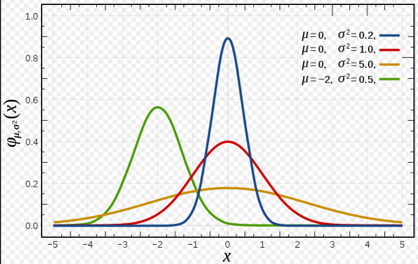
\includegraphics[width=0.7\linewidth]{hustota-pravdepodobnosti}
	\caption{$\Phi(x)$ -- funkce hustoty pravděpodobnosti}
	\label{fig:hustota-pravdepodobnosti}
\end{figure}

\begin{figure}[H]
	\centering
	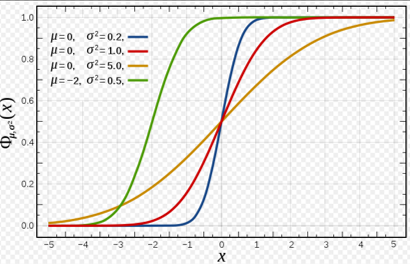
\includegraphics[width=0.7\linewidth]{distribucni-funkce}
	\caption{$\Phi(x)$ -- distribuční funkce (CDF)}
	\label{fig:distribucni-funkce}
\end{figure}

Chybová funkce vyhodnocená pro $\tfrac{x}{\sigma \sqrt{2}}$ (za podmínky normálního Gaussova rozdělení chyb se směrodatnou odchylkou $\sigma$) udává pro absolutní hodnoty $x$ pravděpodobnost, že měření leží ve vzdálenosti menší než $x$ od střední hodnoty.
\begin{figure}[H]
	\centering
	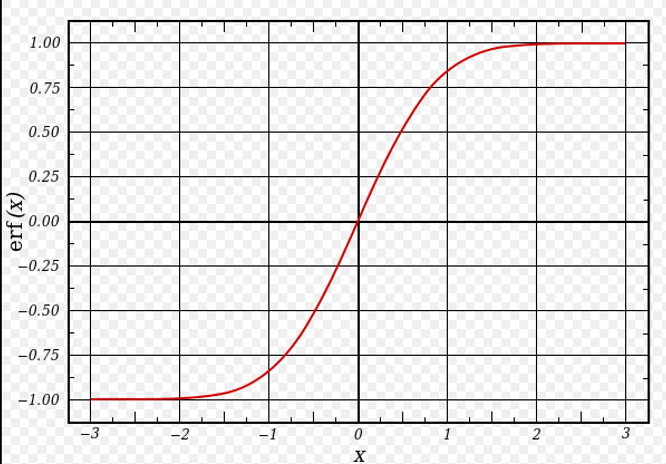
\includegraphics[width=0.7\linewidth]{chybova-funkce}
	\caption{Grafické znázornění chybové funkce}
	\label{fig:chybova-funkce}
\end{figure}

\subsubsection{Matematické vyjádření chybové funkce}
Byla zavedena v~matematice (nazývaná také Gauss error function) je speciální neelementární funkce sigmoidního tvaru, vyskytující se v~pravděpodobnosti, statistice nebo parciálních diferenciálních rovnicích popisujících difuzi.
Je definována takto:
\begin{equation}
	\mathrm{erf}(x) = \frac{2}{\sqrt{\pi}} \int\limits_0^x \exp\left(-t^2\right) \diff t.
\end{equation}

Byla zavedena v~teorii měření (využívající statistiku a~pravděpodobnost) a~název se používá i~při jejím přenosu do jiných oblastí matematiky, které nemají žádný vztah k~charakteristikám chyb měření.

Chybová funkce se vztahuje k~CDF (popisuje prostřednictvím integrálu normálního rozdělení průběh měrné energie napjatosti $\varPhi$) rovnicí
\begin{equation}
	\varPhi(x) = \frac{1}{2} + \frac{1}{2} \mathrm{erf}\left(\frac{x}{\sqrt{2}}\right),
\end{equation}
čímž měníme rozsah hodnot z~intervalu $\langle -1;1 \rangle$ platného pro $\mathrm{erf}(x)$ na interval $\langle 0;1 \rangle$, který platí pro distribuční funkci $\varPhi(x)$.
